\subsubsection{\stid{1.14} UPC++} 
\paragraph{Overview} 
The UPC++ project is developing a C++ library
that supports Partitioned Global Address Space (PGAS) programming~\cite{Bachan:paw17}.
The UPC++ project began in 2012 with a prototype designated V0.1, described in \cite{zheng:ipdps14}.
We are revising the library under the auspices of the DOE's Exascale Computing
Project, to meet the needs of applications requiring PGAS support.
UPC++ is well-suited for implementing elaborate distributed data structures where
communication is irregular or fine-grained. The UPC++ interfaces for
moving non-contiguous data and sending Remote Procedure Calls (RPC)
are composable and closely resemble those used in modern C++.

UPC++ is needed for ECP because it delivers low-overhead communication that runs
at close to hardware speeds, embracing 
interest by vendors in the PGAS model because it 
efficiently matches the RDMA mechanisms offered by
network hardware and on-chip communication between distinct address
spaces.  
Because ECP applications rely on irregular representations
to improve accuracy and conserve memory, the UPC++ library provides
an essential ingredient for the ECP software stack.  It will enable
effective scaling in Exascale software by minimizing the work funneled
to lightweight cores, avoiding the overhead of long, branchy serial
code paths, and supporting efficient fine-grained communication.  The
importance of these properties is exacerbated by application trends;
many ECP applications require the use of adaptive meshes, sparse
matrices, dynamic load balancing, or similar techniques.  UPC++'s
low-overhead communication mechanisms can maximize injection rate and
network utilization, tolerate latency through overlap, streamline
unpredictable communication events, minimize synchronization, and
efficiently support small- to medium-sized messages arising in such
applications.  UPC++ will enable the ECP software stack to exploit
the best-available communication mechanisms, including novel features
being developed by vendors.  This library offers a complementary,
yet interoperable, approach to MPI with OpenMP, enabling developers to
focus their effort on optimizing performance-critical communication.

\paragraph{Key  Challenges}

As the result of technological trends, the cost of data motion is steadily increasing relative to that of computation.  To reduce communication costs we need to 
either reduce the software overheads or hide  communication behind available computation. UPC++ addresses both strategies.
To reduce software overheads, UPC++ takes advantage of the GASNet-EX communication library's \cite{gasnet-spec}
low-overhead communication as well as access to any special hardware
(see the accompanying report on GASNet-EX, which is being co-designed).
UPC++ supports asynchronous communication via classic one-sided communication
(i.e. puts and gets) and remote procedure calls, to support communication hiding.


% A challenge in the ECP-ST effort is to maintain interoperability among run times,
% that invoke the back end to carry out communication. The difficulty is that each
% backend operates under the assumption that it "owns" the network.
% But many ECP applications employ (or will under ECP) multiple runtimes;
% thus interoperability is of paramount concern.
% Our approach is conservative; so long as entries and exits between different
% models is sufficiently coarse grained, then it is feasible to synchronize
% at a barrier at each transition.

\paragraph{Solution Strategy}

The UPC++ project has two primary thrusts:
\begin{enumerate}
\item \textbf{Increased performance through reduced communication costs:} The
UPC++ programmer can expect communication to run at close to hardware speeds.
Asynchronous execution enables an application to hide communication behind
available computation.

\item \textbf{Improved productivity:}  UPC++'s treatment of asynchronous
execution relies on futures and promises, and these simplify the management of
asynchrony.

\end{enumerate}

The PGAS one-sided communication employed by UPC++ (get/put)
benefits application  performance by mapping tightly onto the RDMA
communication supported by the communication network. GASNet-EX provides the
thin middleware
needed to enable this model to run at close to hardware speeds, across platforms ranging from laptops to supercomputers.
One-sided communication also has another benefit.
It decouples synchronization from data motion,
avoiding synchronization overheads of two-sided communication (e.g. message passing).

UPC++'s Remote Procedure Call, which is built on GASNet Active Messages,
provides additional control over asynchronous execution, by enabling
the programmer
to execute procedure calls on remote processors.
RPC is useful in managing access to complicated irregular data structures,
and in expressing asynchronous task execution.

UPC++ addresses productivity via one-sided data motion, remote procedure calls,
and via the provision of futures.
Futures enable the programmer
to capture data readiness state, which is useful in making scheduling decisions, 
via continuations, to execute asynchronously as dependencies become
satisfied. Chaining and conjoining
of asynchronous operations simplify treatment of their completion.



\paragraph{Recent Progress}

symPACK is a direct linear solver for symmetric positive definite sparse matrices.
Originally written using the legacy UPC++ V0.1, we have recently ported symPACK to
use the latest release of UPC++ V1.0. Our experiments conducted on NERSC Edison
confirm that the new UPC++ version preserves the performance of the symPACK solver.


\begin{figure}[htb]
%  \captionsetup{format=centering}
	\centering
	%\includegraphics[width=6in]{sympack-perf}
  \subfloat[\textbf{Push} -- MPI two-sided communication\newline\textbf{Pull} -- UPC++: RPC + RMA Get when ready\newline 2 variants with and without event driven scheduling]{
    \label{fig:sympack:comm}
	  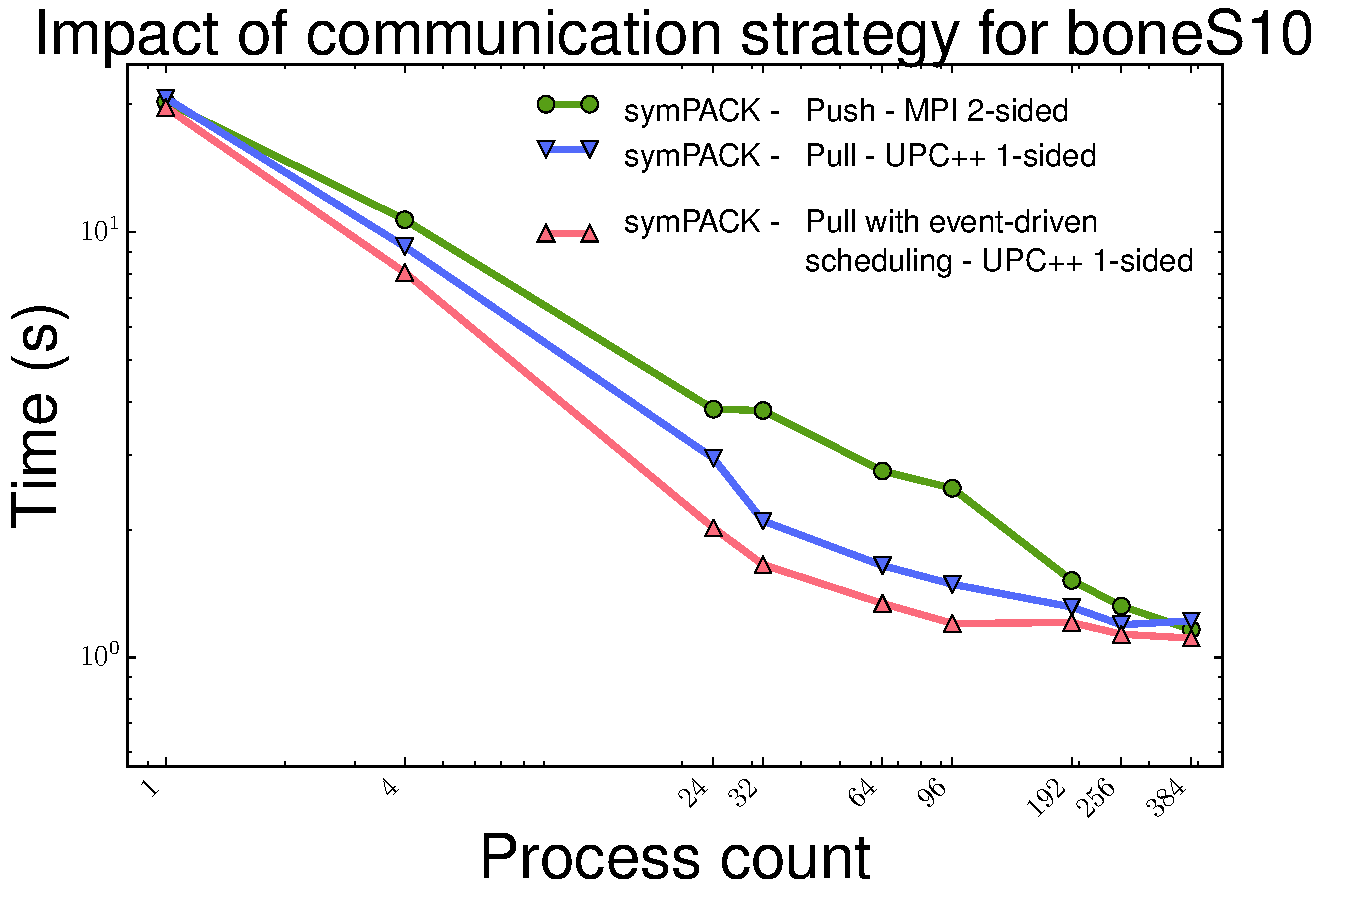
\includegraphics[width=3in]{projects/2.3.1-PMR/2.3.1.14-UPCxx-GASNet/ss_boneS10_comm.pdf}
  }
  \subfloat[Strong scaling of symmetric solvers\newline(Factorization time only)]{
    \label{fig:sympack:scaling}
	  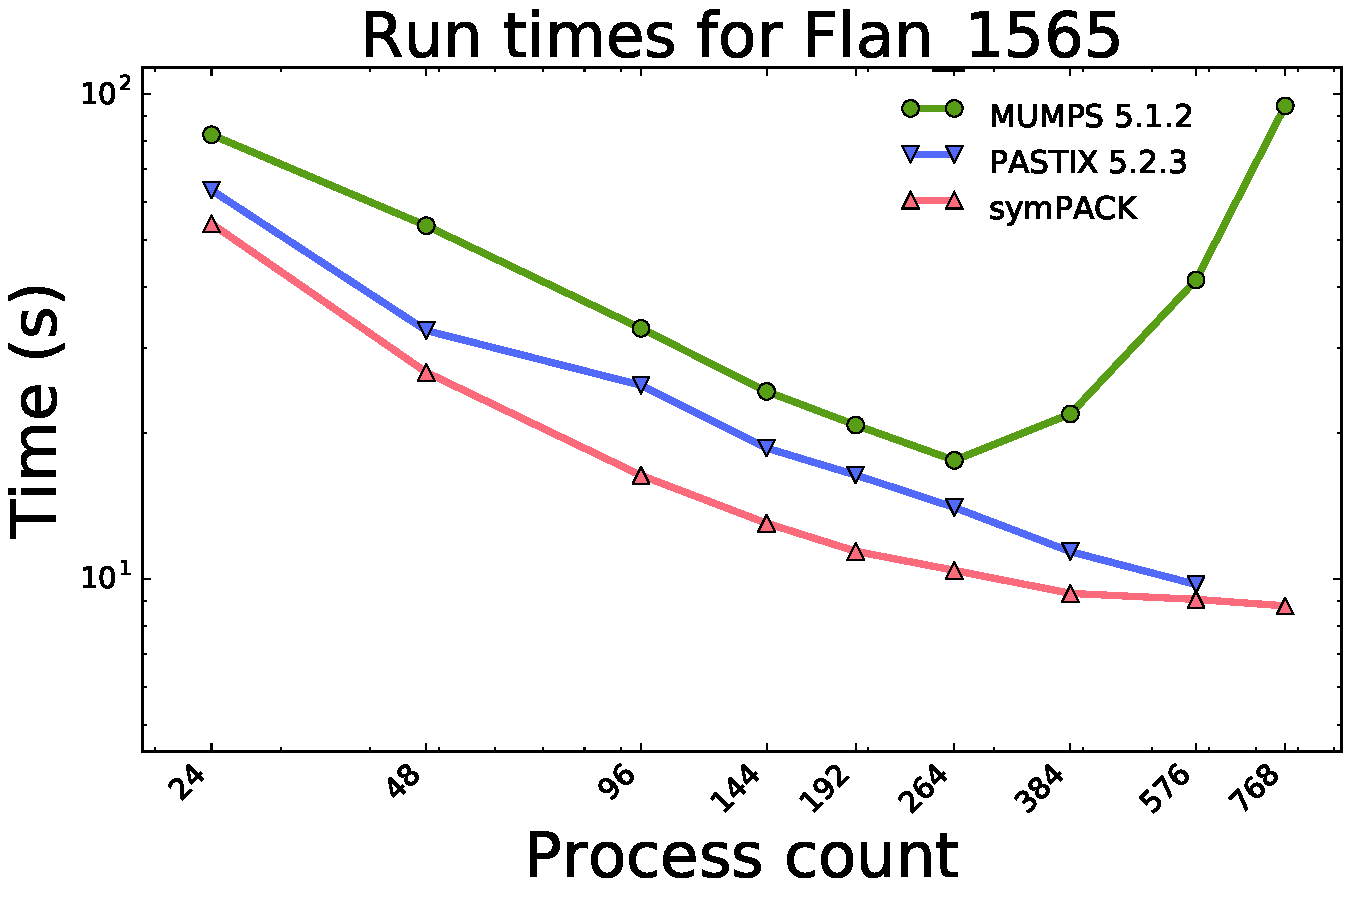
\includegraphics[width=3in]{projects/2.3.1-PMR/2.3.1.14-UPCxx-GASNet/ss_Flan_1565_complex.pdf}
  }
  \caption{\label{fig:sympack-perf}\textbf{Performance of the symPACK solver using UPC++ V1.0} }
\end{figure}



The first experiment, depicted in Fig.~\ref{fig:sympack:comm} compares the performance of three implementations of symPACK:
\begin{itemize}
  \item a \textbf{Push} strategy (the sender ``pushes'' the outgoing message
as soon as possible) using non-blocking MPI two-sided messages,
  \item a \textbf{Pull} strategy (sender ``notifies'' with RPC, receiver RMA gets when ready) using one-sided UPC++ RPC and RMA get,
  \item the same \textbf{Pull} strategy using one-sided UPC++ RPC and RMA get, combined with an event-driven dynamic scheduling policy.
\end{itemize}
UPC++ allows symPACK to implement an efficient Pull strategy using one-sided operations in a simple and efficient fashion.
This implementation surpasses the performance of the original MPI two-sided variant.
Fig.~\ref{fig:sympack:scaling} compares the strong scalability, on NERSC Edison, of symPACK with other state-of-the-art solvers
for sparse symmetric matrices. symPACK can be seen to significantly outperform
the other solvers on this particular problem, a trend which can be observed on most matrices from the SuiteSparse
matrix collection.

%Figure~\ref{fig:sympack-perf} illustrates the benefits of the PGAS model implemented by UPC++ (Mathias' results) .


% Figure~\ref{fig:dht-perf} illustrates the benefits of UPC++'s remote atomics capability with a distributed hash table implementation.
% \begin{figure}[htb]
	% \centering
	% \includegraphics[width=6in]{dht-perf}
	% \caption{\label{fig:dht-perf} {\bf CAPTION GOES HERE STEVE} }
% \end{figure}



\paragraph{Next Steps}


Our next efforts are:
\begin{enumerate}
\item \textbf{Team-aware APIs:} Teams are a mechanism for grouping ranks.
Team-aware APIs  will be developed to enable teams to be used not only in
collective communication (see below) but also in distributed objects,
and certain modes of accessing global shared storage.

\item \textbf{Support for non-blocking collectives:} UPC++ supports a small number
of collectives, and this set will be expanded to accommodate the needs of our
application partners. Support for teams will also be included.
	
	
\end{enumerate}
